%%%%%%%%%%%%%%%%%%%%%%%%%%%%%%%%%%%%%%%%%%%%%%%%%%%%%%%%%%%%%%%%%%%%%%%%%%%%%%%%
%2345678901234567890123456789012345678901234567890123456789012345678901234567890
%        1         2         3         4         5         6         7         8

\documentclass[letterpaper, 12 pt, conference]{ieeeconf}  % Comment this line out if you need a4paper

%\documentclass[a4paper, 10pt, conference]{ieeeconf}      % Use this line for a4 paper

\IEEEoverridecommandlockouts                              % This command is only needed if 
                                                          % you want to use the \thanks command

\overrideIEEEmargins                                      % Needed to meet printer requirements.

% See the \addtolength command later in the file to balance the column lengths
% on the last page of the document

% The following packages can be found on http:\\www.ctan.org
%\usepackage{graphics} % for pdf, bitmapped graphics files
%\usepackage{epsfig} % for postscript graphics files
%\usepackage{mathptmx} % assumes new font selection scheme installed
%\usepackage{times} % assumes new font selection scheme installed
%\usepackage{amsmath} % assumes amsmath package installed
%\usepackage{amssymb}  % assumes amsmath package installed
\usepackage[english]{babel}
%\usepackage[utf8]{inputenc}
%\usepackage{amsmath}
\usepackage{graphicx}
\usepackage{hyperref}
\usepackage{amsmath}

\title{\LARGE \bf
Scalable Algorithms for Natural Language Processing
}

\author{Ryan Butler, Dae Won Kim, Peiyun Zhang}

\begin{document}

\maketitle
\thispagestyle{empty}
\pagestyle{empty}
%%%%%%%%%%%%%%%%%%%%%%%%%%%%%%%%%%%%%%%%%%%%%%%%%%%%%%%%%%%%%%%%%%%%%%%%%%%%%%%%

\begin{abstract}
The standard procedure of creating frequency-count matrix - most commonly referred to as the Document-Term-Matrix(DTM) - for text analysis can pose major challenges to standard machine learning algorithms, because such representations often exhibit high sparsity and very large width-to-height ratios. This makes NLP prone to issues in scalability, overfitting, and inaccurate approximations of optimal solutions. Thus dimensionality reduction and numeric embedding techniques are essential to making text analysis tractable. Our objective is to explore the effects of such techniques on scalability of classification algorithms on the Yelp review classification problem. Specifically, we aim to analyze embedding techniques on their ability to reduce the gap in predictive power between scalable, linear algorithms and more complex, and thus poorly scalable ensemble counterparts.
\end{abstract}


%%%%%%%%%%%%%%%%%%%%%%%%%%%%%%%%%%%%%%%%%%%%%%%%%%%%%%%%%%%%%%%%%%%%%%%%%%%%%%%%
\section{INTRODUCTION}

Yelp is a review-sharing platform, in which users actively archive numeric evaluations of businesses in the form of a star rating and provide context by text. The reviews are then further evaluated by other users, who can choose to tag each review post as "funny","cool", or "useful". 

\begin{figure}[h]
	\centering
	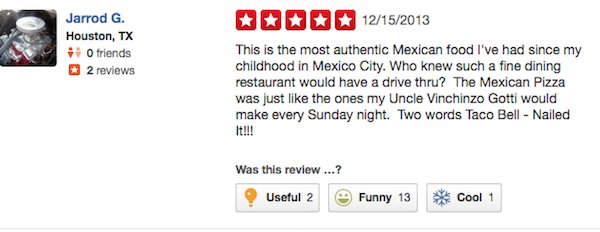
\includegraphics[scale=0.45]{yelp_review.jpg}
	\caption{Yelp Review Example}
    \label{yelp_review}
\end{figure}

The accumulation of such votes can illustrate the "character" of each review. Analyzing the relationship between the contents of the review and these votes can reveal what determines one's reaction to a block of text and its context. Broadly, such analysis is akin to sentiment analysis, in which positivity of a block of text can be mapped to a numeric scale representing positivity. Our problem then is to classify whether each review can be classified as either "funny", "cool", or "useful." However, these three categories are more complex constructs and not mutually exclusive. Our challenge, therefore, rests on how we define our target predicted variable, and on finding an effective numeric embedding of the text data. In particular, our aim is to analyze the effectiveness of text-to-numeric transformation techniques in bridging the gap between linear, scalable ML models, such as logistic regression, to poorly scalable complex models, such as random forest, in predicting funny, cool, or usefulness of Yelp reviews.

\section{Data Preprocessing}

\subsection{Data Acquisition}
\begin{table}[h]
	\centering
	\begin{tabular}{l l l}
		\hline
		\textbf{Column Name} & \textbf{Type} & \textbf{Description}\\
		\hline
		review\_id & string & unique review id \\
		stars & integer & average star rating for a review\\
		text & string & review text (typically 200+ words)\\
		useful & integer & number of useful votes received\\
		funny & integer & number of funny votes received\\
		cool & integer & number of cool votes received\\
		\hline
	\end{tabular}
	\caption{Review Dataset Schema}
\end{table}
Data was obtained from the \href{https://www.yelp.com/dataset/challenge}{Yelp Dataset Challenge}, which offers several large files that respectively contain information on $4$ million reviews, $1$ million users who wrote these reviews, and $150,000$ businesses. All of our operations for this midterm report were done exclusively on the review file. The dataset also contains ids that connect it to the author and business, associated star rating, date of authorship, and votes made by other users. However, our focus in this project was text analysis, and non-textual information was therefore excluded. Shown above is the schema of the review dataset used for analysis(Table 1).

\subsection{Subsetting the Data}
In order to make the dataset more manageable and improve model accuracy, we filtered the dataset to fit our needs. In particular, we wanted to filter out reviews that were ambiguous in the category they fell in. The less the ambiguity, the more likely our ML models should perform. However, the trade-off is in loss of data and information. After a certain filter threshold value, the model accuracy offered by accepting only highly skewed data would lead to overfitting, making it necessary to preserve a minimum amount of data.

In particular, we filtered by two parameters: a minimum number of compliments and a minimum ratio of the largest compliment type to the total number of compliments. This ensured that we could filter out noise that would arise from reviews with too few compliments, and also filter out reviews that were ambiguous about which class they resided in.

\begin{figure}[h]
	\centering
	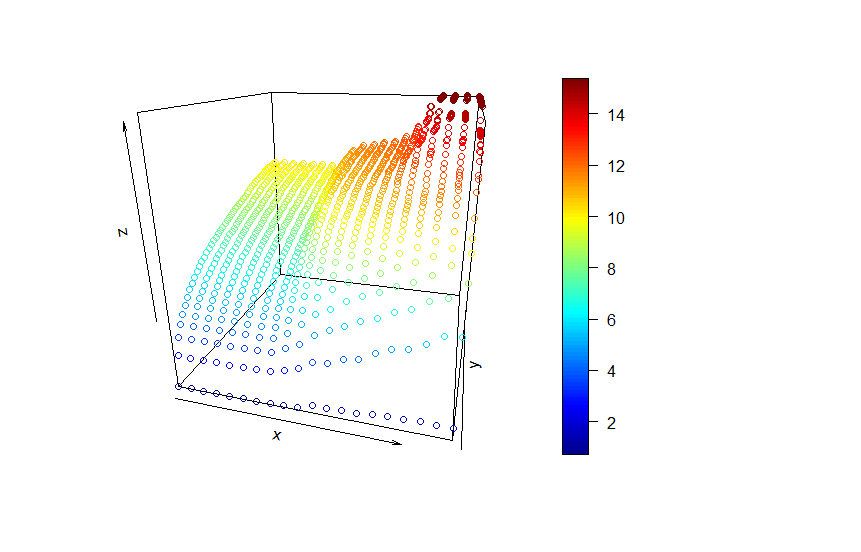
\includegraphics[scale=0.45]{3d_plot.png}
	\caption{Grid Search of Filter Parameters}
    \label{param_search}
\end{figure}

Figure \ref{param_search} shows a plot of the logged percentage of reviews filtered out as a function of the filter conditions we apply. Using this plot as a guide, we decided to choose a value of $10$ as the minimum acceptable number of total votes. This ensures that sample size is enough to make it a representative sample of people who would ever come across this review. \\For the ratio parameter, we found that there was a very large change in the number of reviews filtered out on the interval $[0.4, 0.5]$, where the reviews ranged from over $100,000$ to just over $30,000$. This meant that going any higher than $0.5$ for the threshold would filter out dramatic amounts of data. This is the reason why we decided to go with $0.4$, which held roughly $128,000$ rows, a number we believed to be a good compromise between data size and separability of classes. 

\subsection{Text Data Processing}
We first conducted \href{https://www.ibm.com/developerworks/community/blogs/nlp/entry/tokenization?lang=en}{tokenization} on each of the review text in the data. Tokenization is a process typically denoting the splitting of sentences and phrases into its individual parts. 
$$\text{this is a sentence} \Rightarrow \text{this},\text{is},\text{a},\text{sentence}$$

Then, we applied \href{http://language.worldofcomputing.net/pos-tagging/parts-of-speech-tagging.html}{speech tagging} onto to words token we created in the previous step.Speech tagging, or parts-of-specch tagging is a technique we used to automatically assign descriptors to given word tokens. 
$$\text{Pizza } \text{to } \text{Noun}, \text{Delicious } \text{to } \text{Adjective}$$

The tagging helps with the next step, where very similar words, or words with shared roots are binned together in a process known as normalization. Stemming, the first normalization techniques we considered, basically takes a word and cuts off the end part of the world to achieve normalization. It does so by matching patterns like "s", "es","ed" and so on. The simplicity of this approach makes it efficient. 
$$\text{takes}, \text{taken}, \text{taking}  \Rightarrow \text{take}$$

However, one disadvantage of this technique is that due to many exceptions, a pattern-matching set of rules bound to have many exceptions. This results in many words losing meaning after being stemmed. Therefore, we decided to use lemmatization, which tries to locate the core-meaning rather than through a pattern matching system, as shown in the example below.
$$\text{faster}, \text{fastest},\text{quickly} \Rightarrow \text{fast}$$

We then remove stop words. Stop words are words appear at a relatively high frequency but do not have any meaning in text analysis such as "the", "a" and "that".This is aimed to strip away words that dominate in frequency but hold little meaning without context.
$$\text{this}, \text{is}, \text{a}, \text{sentence} \Rightarrow \text{sentence}$$

\subsection{Text-to-numeric Transformation}
Once the text has been reduced by applying aforementioned preprocessing techniques, the frequency of each word is counted for each review, and stored as rows of a frequency-count matrix, or a Document-Term-Matrix (DTM) Initially this matrix had more than $200,000$ columns. We sorted our vocabulary by the total number of times used in the dataset, and choosing the top $100,000$. This number was used because it was lower than the number of data points: $128,000$. This DTM was used to fit ML models initially to establish a baseline benchmark to compare our more advanced embedding techniques.

For more advanced numeric encoding of text information, we used \href{https://en.wikipedia.org/wiki/Word2vec}{Word2vec}, a popular word embedding framework initially developed by Google. It transforms a DTM using a low-dimensional vector space created by a two-layer neural network.The neural network performs a non-linear mapping between the original vocabulary space, to a newly transformed feature space that can cluster similar words together in location and orientation. To offer a high-level overview, the word2vec produces from a block of text its "orientation" based on a shared vocabulary space. The resulting numeric matrix - made by row-wise concatenation of word2vec transformations - is a reflection of the similarities in certain words in their use cases, as will be later shown in a visual.

\section{Exploratory Analysis}

\subsection{Data Visualization}

The two filtering principles reduces the 4 million reviews to about $128,000$ reviews, which is less than $30\%$ of the data we started with. Overall, usefulness is the most dominant of these categories, with at least $70\%$. We wanted to see if there are obvious factors other than the text that affects voting intensities in the three categories. Figure \ref{vote_cate} is the box plot of number of maximum vote for each review grouped by is associated category. From this plot, it is quite obvious that within "useful", negative reviews tend to have higher votes; whereas positive reviews tend to have higher votes within "funny" category. Yet "cool" does not appear to be a popular button at all. Also in general, "useful" receives far more votes than "funny" and "cool" combined. This suggests that the star rating of a review may be a significant factor in determining the perception of usefulness, coolness, or funniness.

\begin{figure}[h]
	\centering
	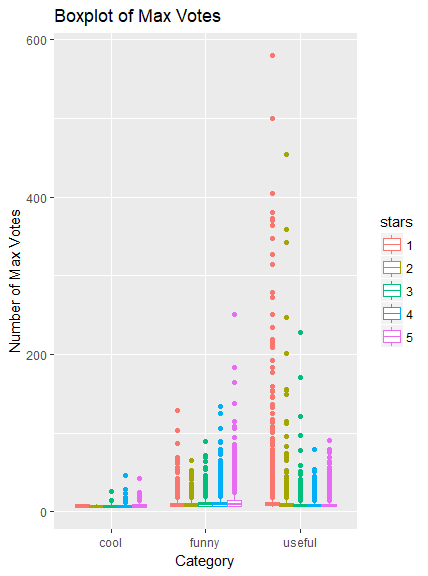
\includegraphics[scale=0.50]{vote_category_boxplot.png}
	\caption{Boxplot of Max Votes}
    \label{vote_cate}
\end{figure}

\subsection{Principal Component Analysis}
To understand the behavior of the vocabulary space represented by the DTM, principal component analysis (PCA) was used. PCA is useful in establishing a baseline transformation technique, since it is one of the simpler transformation of its kind. Unlike word2vec, PCA is a linear transformation technique, and thus is expected to behave relatively poorly in word spaces. Figure \ref{pca_var} shows the explained variance quickly decays to below $0.1$ by the third component. This suggests, among other things, confirms the extremely high sparsity of the vocabulary space, as well as the low-rank structure. This means overall the data is only highly variant on certain directions or subspaces, and overall very clumped together. This is completely in line with expectations given that this structure completely ignores latent structure in language where context, similarity, sequence, and meaning is not necessarily factored in. Also indicated some significant correlation between the words, which is expected, since set of words used from person to person is most likely very highly correlated. 

\begin{figure}[h]
	\centering
	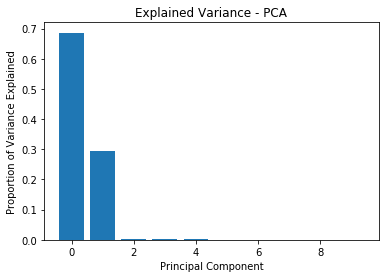
\includegraphics[scale=0.53]{pca_var.png}
	\caption{PCA Explained Variance}
	\label{pca_var}
\end{figure}

To further visualize, first three principal components were then plotted onto a 3D space, in order to visualize whether certain clumping does occur. Figure \ref{w2v_3d} is the result. The colors represent associated category. There is low degree of separability between the three colors, as suspected. It may be noted, however, that some amount of green does seem to congregate on the right upper side more, and brown color congregates more on the lower left, and yellow overall populating the center (yellow dominates as it represents usefulness, which is $70\%$ of the data). This peculiarity in the distribution gives some indication as to separability in a higher dimension space. \\

\begin{figure}[h]
	\centering
	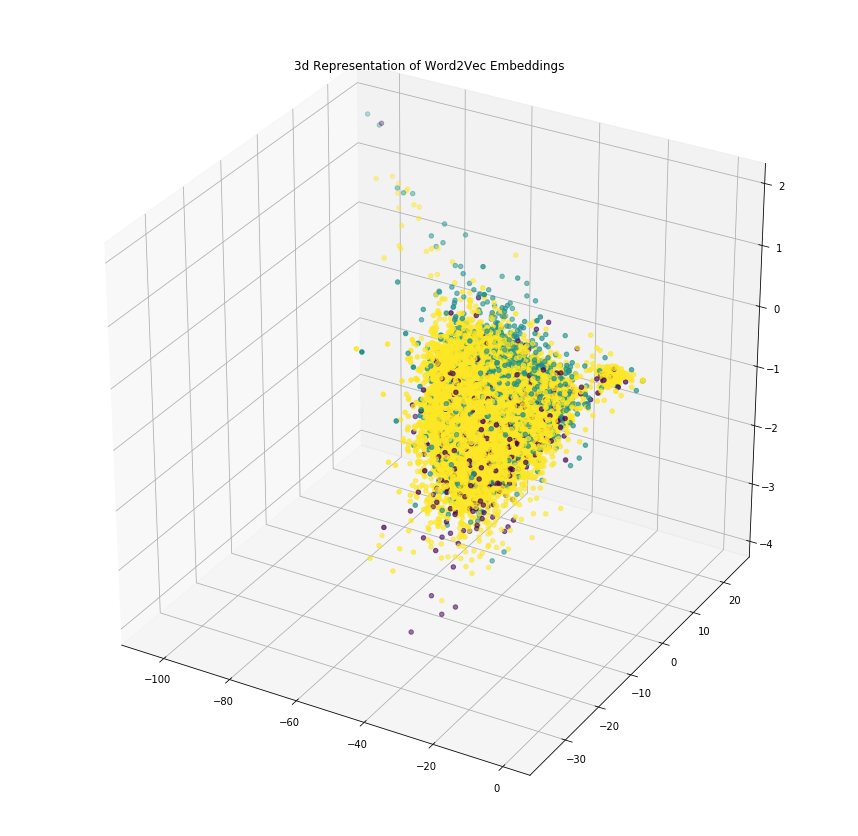
\includegraphics[scale=0.25]{word2vec_3d.png}
	\caption{PCA 3D Representation}
    \label{w2v_3d}
\end{figure}

Another visualization technique for high dimensions is the t-distributed stochastic neighbor embedding \href{https://lvdmaaten.github.io/tsne/}{(t-SNE)}, which does relatively well in preserving high-dimensional distances in low dimensional projections through a process called "ex (usually two or three dimensions). This lower dimension space can then be visualized in a scatter plot, which usually provides a clear pattern of classification.

\begin{figure}[h]
	\centering
	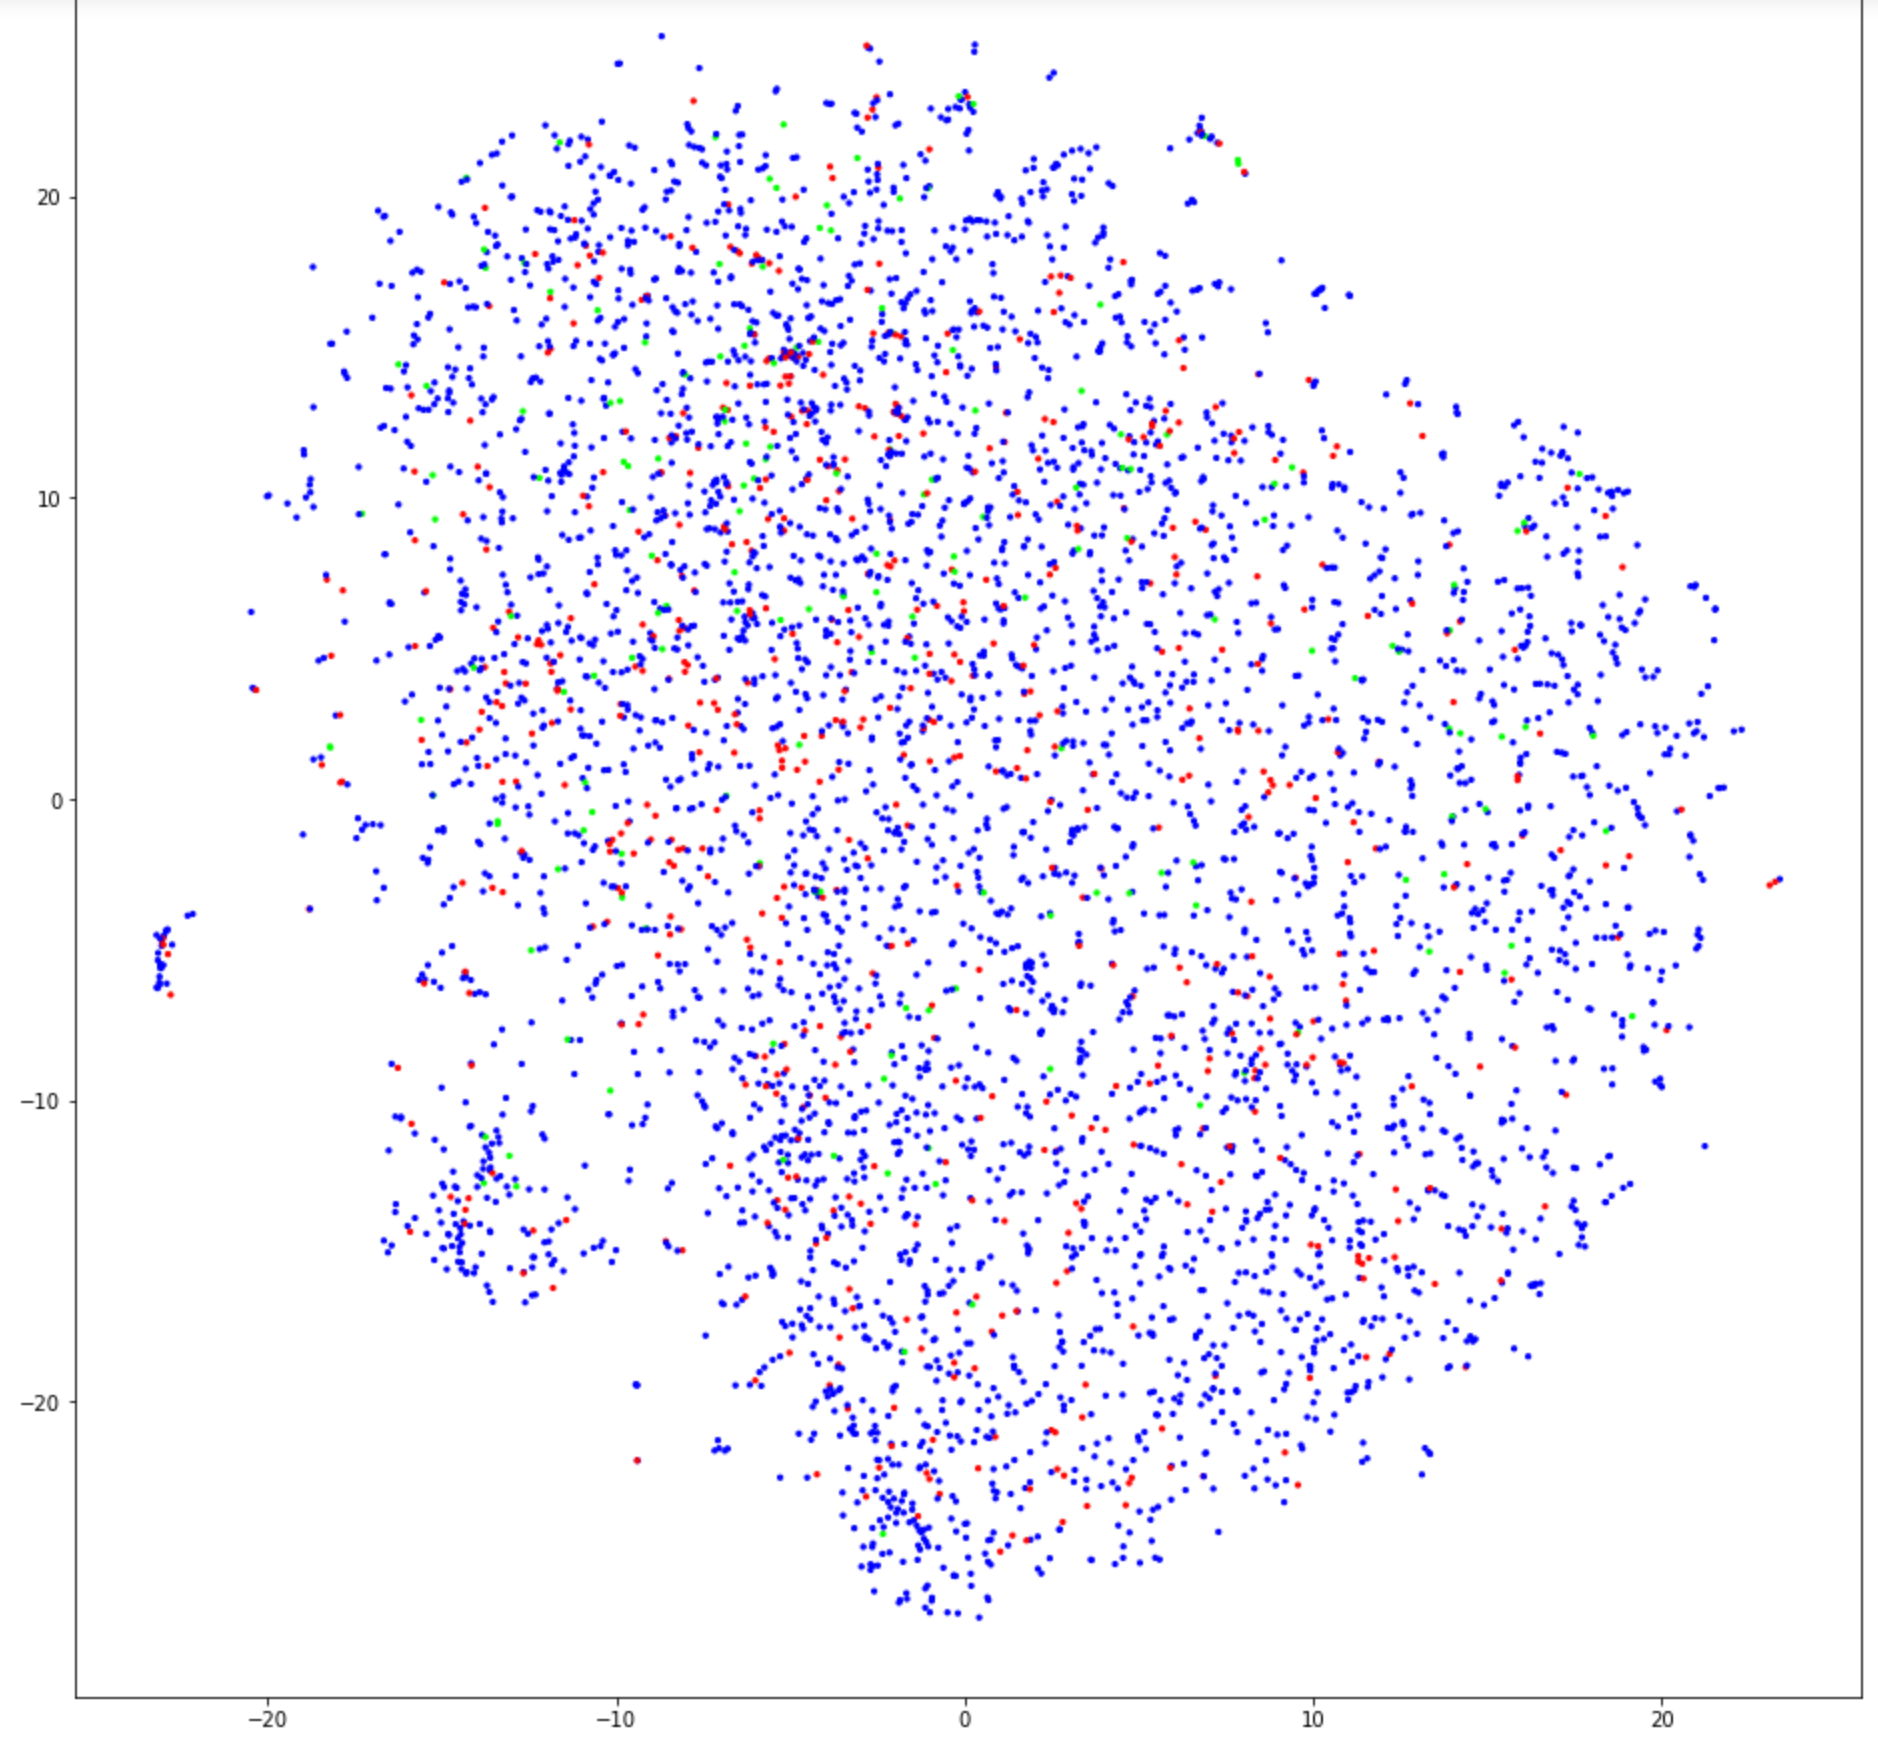
\includegraphics[scale=0.1]{dtw_tsne.png}
	\caption{Document Term Matrix t-SNE}
    \label{dtm_tsne}
\end{figure}

Figure \ref{dtm_tsne} shows a relatively unclustered, uncharacteristic space. However,in Figure \ref{w2v_tsne}, it is clear that the data has become more separable. This shows that word2vec indeed 'clumps' similar regions of the words together.

\begin{figure}[h]
	\centering
	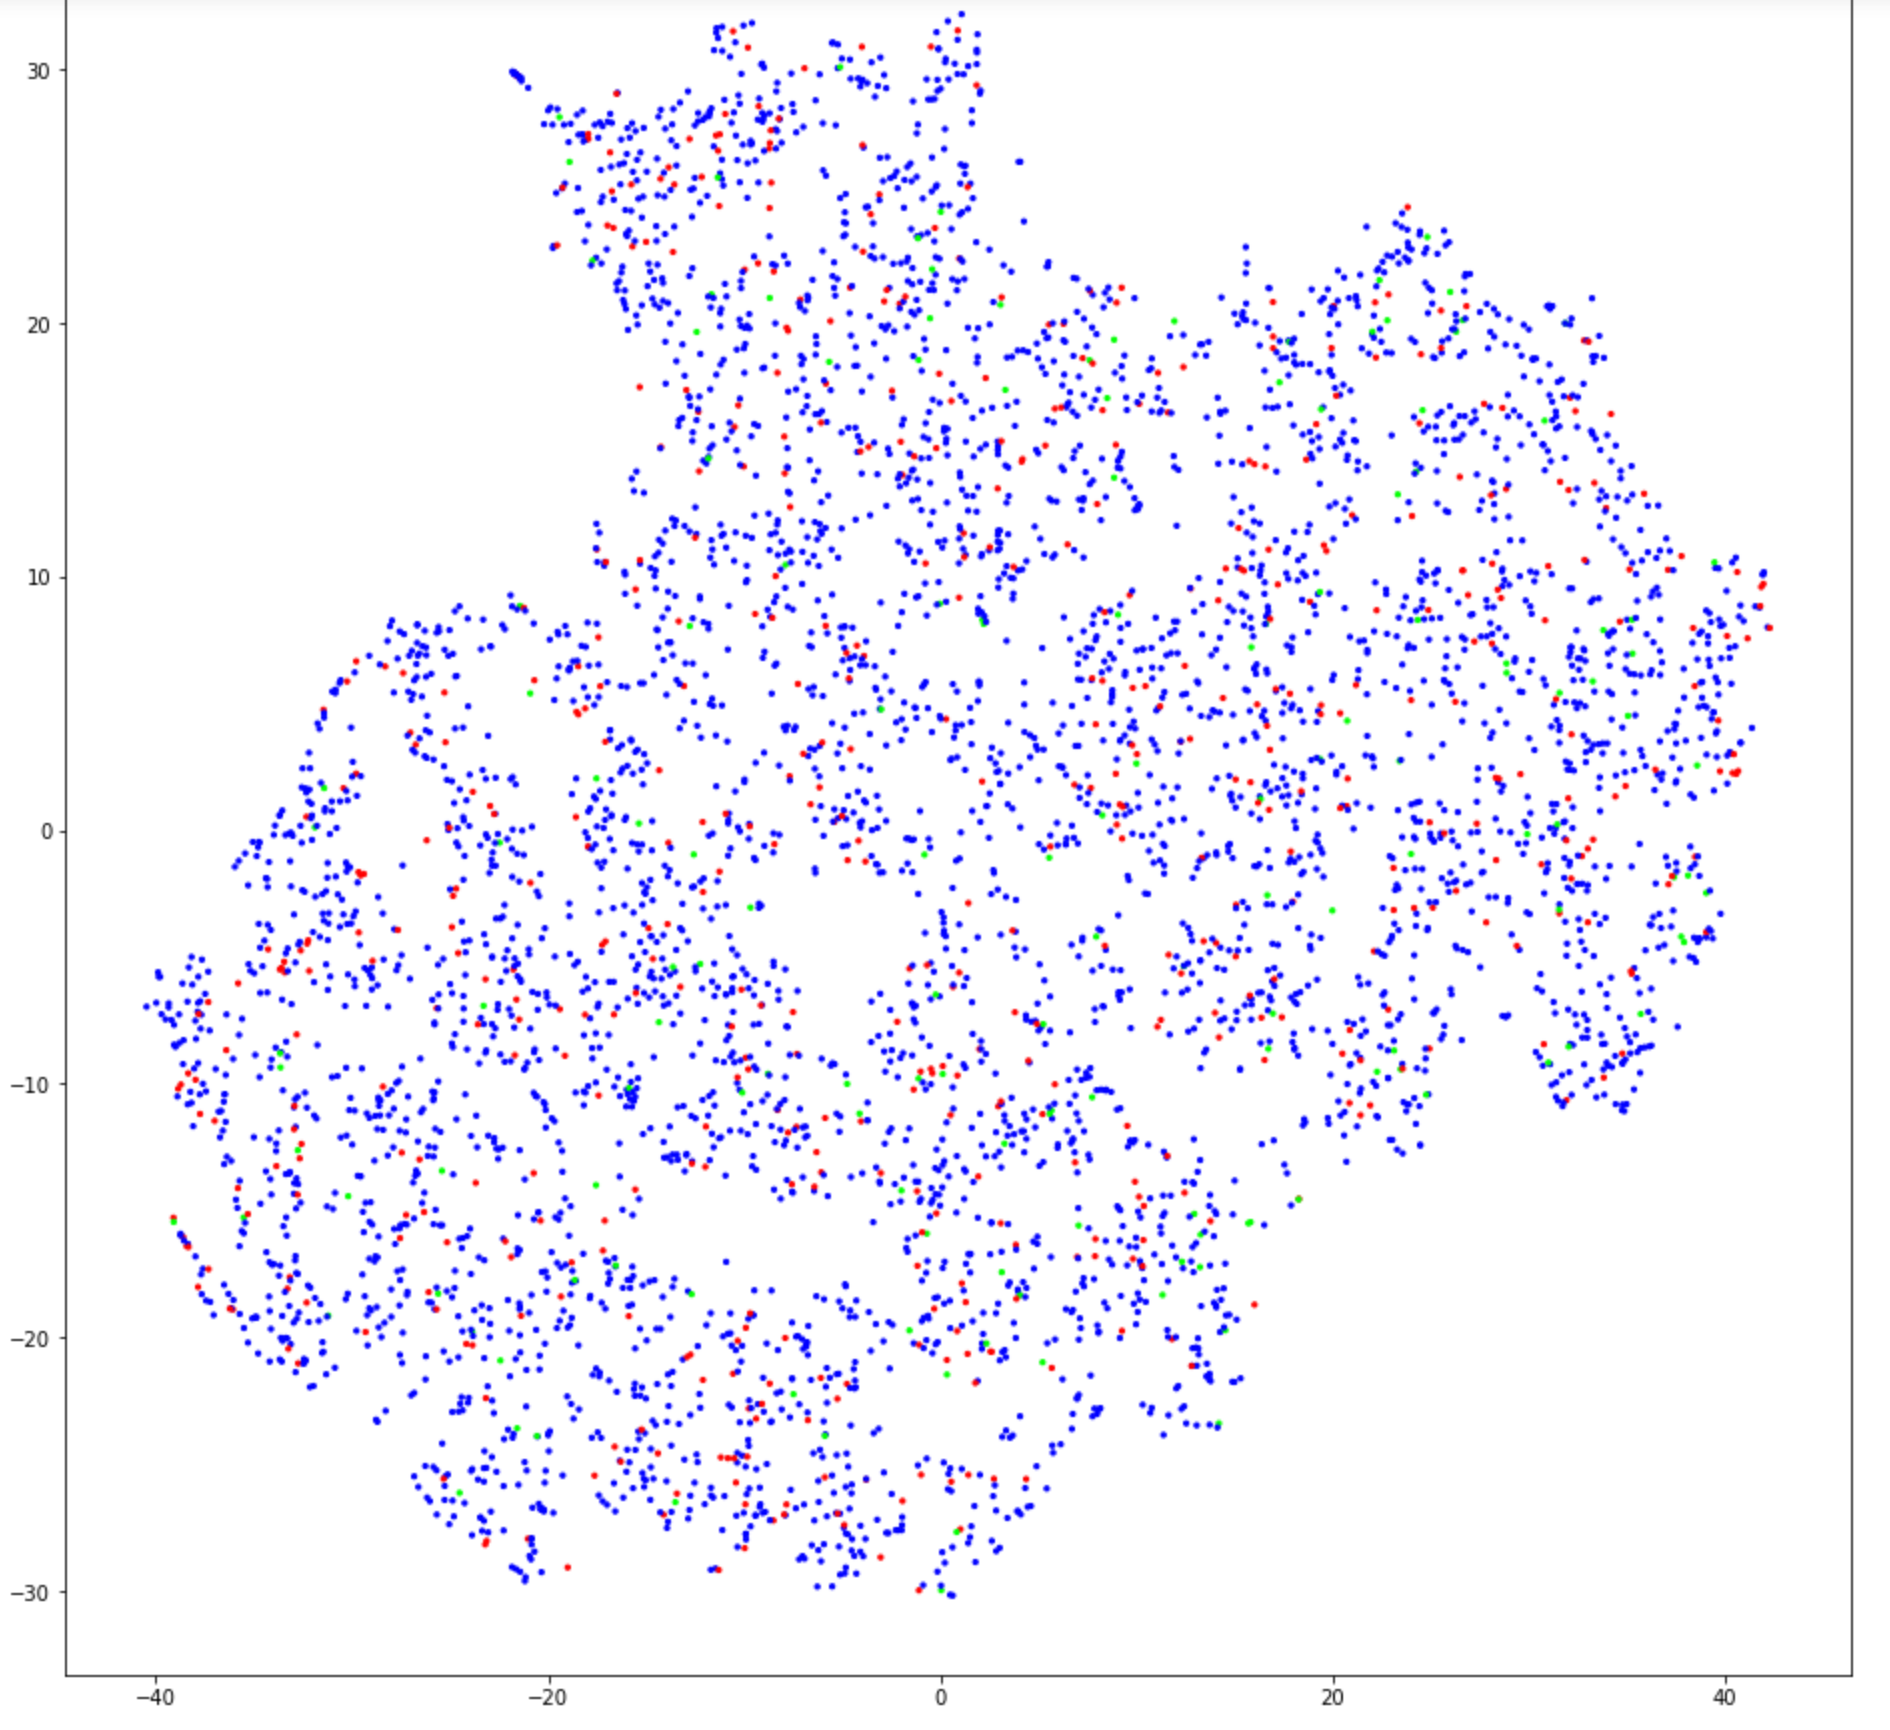
\includegraphics[scale=0.1]{word2vec_tsne.png}
	\caption{Word2Vec t-SNE}
    \label{w2v_tsne}
\end{figure}

\section{Evaluation Method}
\subsection{Model Evaluation}
We used $F_1$ score as the error metric to measure the prediction accuracy. The F1 score is a popular weighted accuracy metric for multiclass-classification problem, since our output space is defined as three categories. $F_1$ score takes both the precision $p$ and the recall $r$ of the test into consideration in computing the score. More specifically,  $p$ is the true positive rate and $r$ is the number of correct positive results divided by the number of positive results that should have been returned. The formula is $$F_1 = 2 \times \frac{1}{\frac{1}{r}+\frac{1}{p}} = 2 \times \frac{p\times r}{p + r}$$ As a result, the closer $F_1$ gets to $1$, the better the prediction result will be.

We then used cross validation - specifically 5-fold validation - to allow maximal use of the training set, while also making sure our error metric is not prone to overfitting to the training set. How we also avoid overfitting by controlling bias is mentioned in the next section.
\subsection{Bias and Variance control}
Word embeddings can be prone to overfitting due to the high correlation between the dimensions, and the high dimensionality of the space. This problem, while lessened by the use of embeddings, does not necessarily completely disappear. Therefore for all our models we incorporated regularizations such as L1 and L2 regularization loss, or pruning. It is important to note that in this case L2 is the more suitable candidate because L1 regularizer tends to push coefficients to zero, while the word embedding dimensions are usually compressed information on the original vocabulary space and would result in further information loss. That was why L2 regularizer was generally preferred Further dimensionality reduction from our word2vec transformation seems unnecessary, however, because we have 128,000 data points and 128 as our word2vec output dimension. and may result in underfitting. 

\section{Analysis}

The next figure shows the distribution of the words for the top 10 words. As expected of language, it displays a heavy-tail pareto distribution. The decay is not as abrupt because we have removed stop words, which would have greatly skewed the data. It is interesting how these words are seemingly very common, and maybe indicative of the fact that high-frequency counts may not necessarily correlate with importance.
\begin{figure}[h]
	\centering
	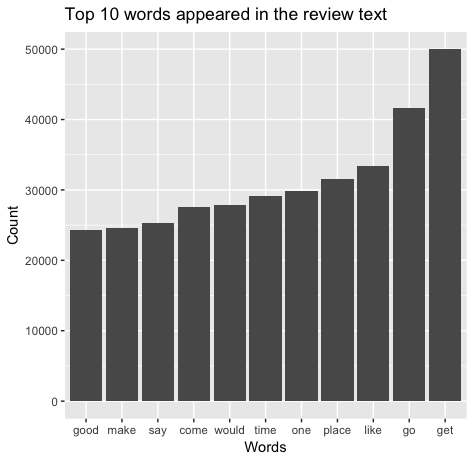
\includegraphics[scale=0.53]{word_count.png}
	\caption{Barplot of Word Count}
    \label{word_count}
\end{figure}

After cleaning and embedding all of our filtered data, we fitted our data into three classification models: multinomial logistic regression - which uses softmax loss to compute the probabilities for the three classes and chooses the maximum value - , decision tree which uses cross-entropy loss, and random Forest, which is a tree ensemble with subset selection. Logistic regression is the linear, scalable model, while decision tree is considered to be non-linear and also relatively less scalable. Random Forest is on the more extreme end of poor scalability, but carry  In each of the method, we applied 5-fold cross-validation to ensure the validity of our analysis. 
\begin{figure}[h]
	\centering
	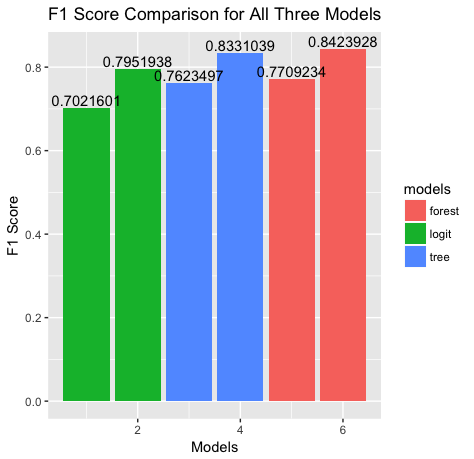
\includegraphics[scale=0.5]{model_comparison.png}
	\caption{Model Comparison}
    \label{model_comparison}
\end{figure}

This graph displays the improvement word2vec offers for the three algorithms. each color represents logistic regression, decision trees, and random forest. The bar on the left is with just the DTM, and the right after embedding. As can be seen, Word2vec indeed brings significant improvements to all three algorithms. The three of them are, as expected, have F1 scores correlated with their relative complexity. however, it is noticeable that the gap between logistic regression and the rest have narrowed noticeably, due to the fact that logistic regression's growth in accuracy has been largest.

\subsection{Logistic Regression}
As we have three categories in the output space, we used multinomial logistic regression, which applies the softmax loss, which is a general case of the logit function to multi-class output space.The regularization parameter used was L2. As shown in Figure \ref{logit_plot}, the function simply decays exponentially, suggesting that the model as expected is still grossly underfitting, It reaches maximum F1 score of $0.79$ with the use of word2vec, while only $0.7$ without.
\begin{figure}[h]
	\centering
	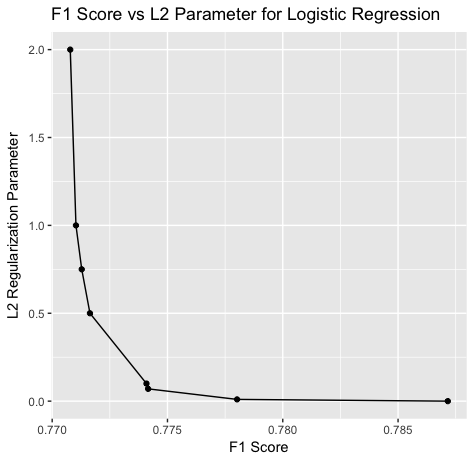
\includegraphics[scale=0.5]{logit_plot.png}
	\caption{Logistic Regression Result}
    \label{logit_plot}
\end{figure}

\subsection{Decision Tree}
We controlled the number of tree at 100 and fit decision tree model with different max depths along with the Cross-entropy loss. As shown in \ref{dt_results}, the F1 score first increases then decreases as we increase the max depths with a small fluctuation in the middle. The F1 score peaks when max depths is $10$. We also observed an increase in the F1 score after applying word2vec, which changes from $0.76$ to $0.83$ 
\begin{figure}[h]
	\centering
	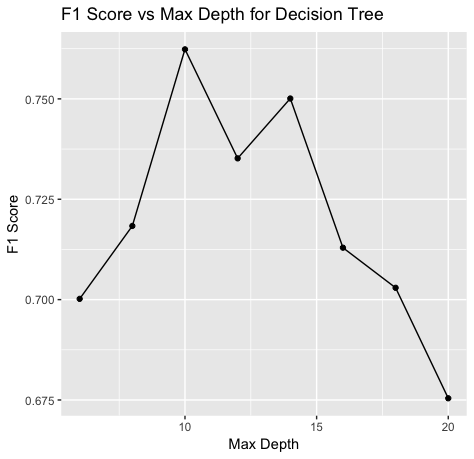
\includegraphics[scale=0.4]	
    {dt_result.png}
	\caption{Decision Tree Results}
    \label{dt_results}
\end{figure}

\subsection{Random Forest}
Another tree-based model we used to train out model is random forest. This is an ensemble method for classification as it repetitively randomly select a certain number of predictors from the input space. Therefore, the result does not always follow the stronger predictors in the input space as decision trees does. In this sense, random forest is efficient in reducing model variance. We set the number of trees as $100$, and fit the random forest model with different max depths. As shown in Figure \ref{rf_result}, the F1 score first first increases and peaks when max depths is 10, then rapidly decreases as the max depths further increase. The result shows that applying word2vec increased F1 score from $0.77$ to $0.84$.

\begin{figure}[h]
	\centering
	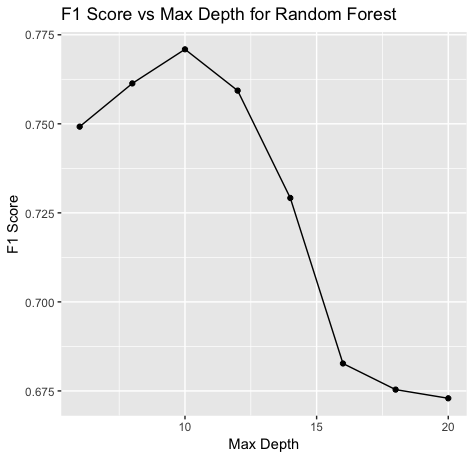
\includegraphics[scale=0.4]		
    {rf_result.png}
	\caption{Random Forest Results}
    \label{rf_result}
\end{figure}

\subsection{Limitations}
To process very large text files - gigabytes of it - Apache Spark was used. It comes with modules on text processing, principal component analysis, and allows scalability of algorithms. We also had access to a Linux cluster with 70 cpu cores, which further improved our computing performance. Most of the preprocessing code was done using regular python, particularly the json and nltk. However this did impose some limitations on what functions and loss functions we could use. For example, L2 loss is much more conducive to parallelism because it is differentiable and convex, leading to gradient descent methods which are very much easy to parallelize. However L1 loss usually not used for models because it usually requires subgradient descent or the Huber loss, which can have unstable paths and inaccurate final solutions, which is not as conducive to parallel platforms such as Spark. Therefore our focus in variation lies in complexity control measures such as terminating conditions, tree-depth, and regularization measures. 

\section{Conclusion}
We were able to conclude that text embeddings not only actually make accuracy of models generally better - which was very much expected - it also bridges the gap in predictive power between linear and non-linear models. While this may seem like an obvious consequence of the non-linearity of the embedding itself, it is surprising that it more positively affects the linear more so than the non-linear ones. This suggests that linear models tend to grossly underfit the space in vocabulary, while more complex methods either overfit or are flexible enough to incorporate latent structure in language.We trained our own word2vec, rather than using pretrained ones, and realize that pretrained ones most likely can do a lot better, since oftentimes they have other data sources to confirm their effectiveness in algorithm improvement. We have been able to learn much on the importance of unsupervised learning methods in the context of preparing the data for supervised learning problems. 
\end{document}
